\chapter{Methods}

\section{Toolchain}

The whole project can be summarized in four single steps or tasks:
\begin{enumerate}
	\item Data: Collect a dataset, for inference, for training and for testing
	\item Model: Get to know at least one model, for inference and for retraining
	\item Tidy: For a given input picture, return an image that displays a repertoire of all found objects in the input picture
	\item App: Turn the former three tasks into an application that can be reached from a web browser.
\end{enumerate}

In order to develop a minimal viable product, all these four tasks have to be solved first. The way of proceeding was to develop a minimal viable product first and then to start with refining the model and adjusting the app. This means going through the full circle first, before adjustments and proceeding into retraining are made.

\section{Project management}

In the beginning of the project, a project management plan had to be developed. The project management plan contains a timeline with all (then known) tasks and a list of all milestones. Trello together with a timeline add-on (a gant chart) was used as project management toool. The project management plan and all tasks and milestones can be seen via this link: \url{https://trello.com/b/srqnMstX/object-detection-in-fine-art-photography}. A picture, showing the full timeline is shown here:

 \begin{figure}
	\center{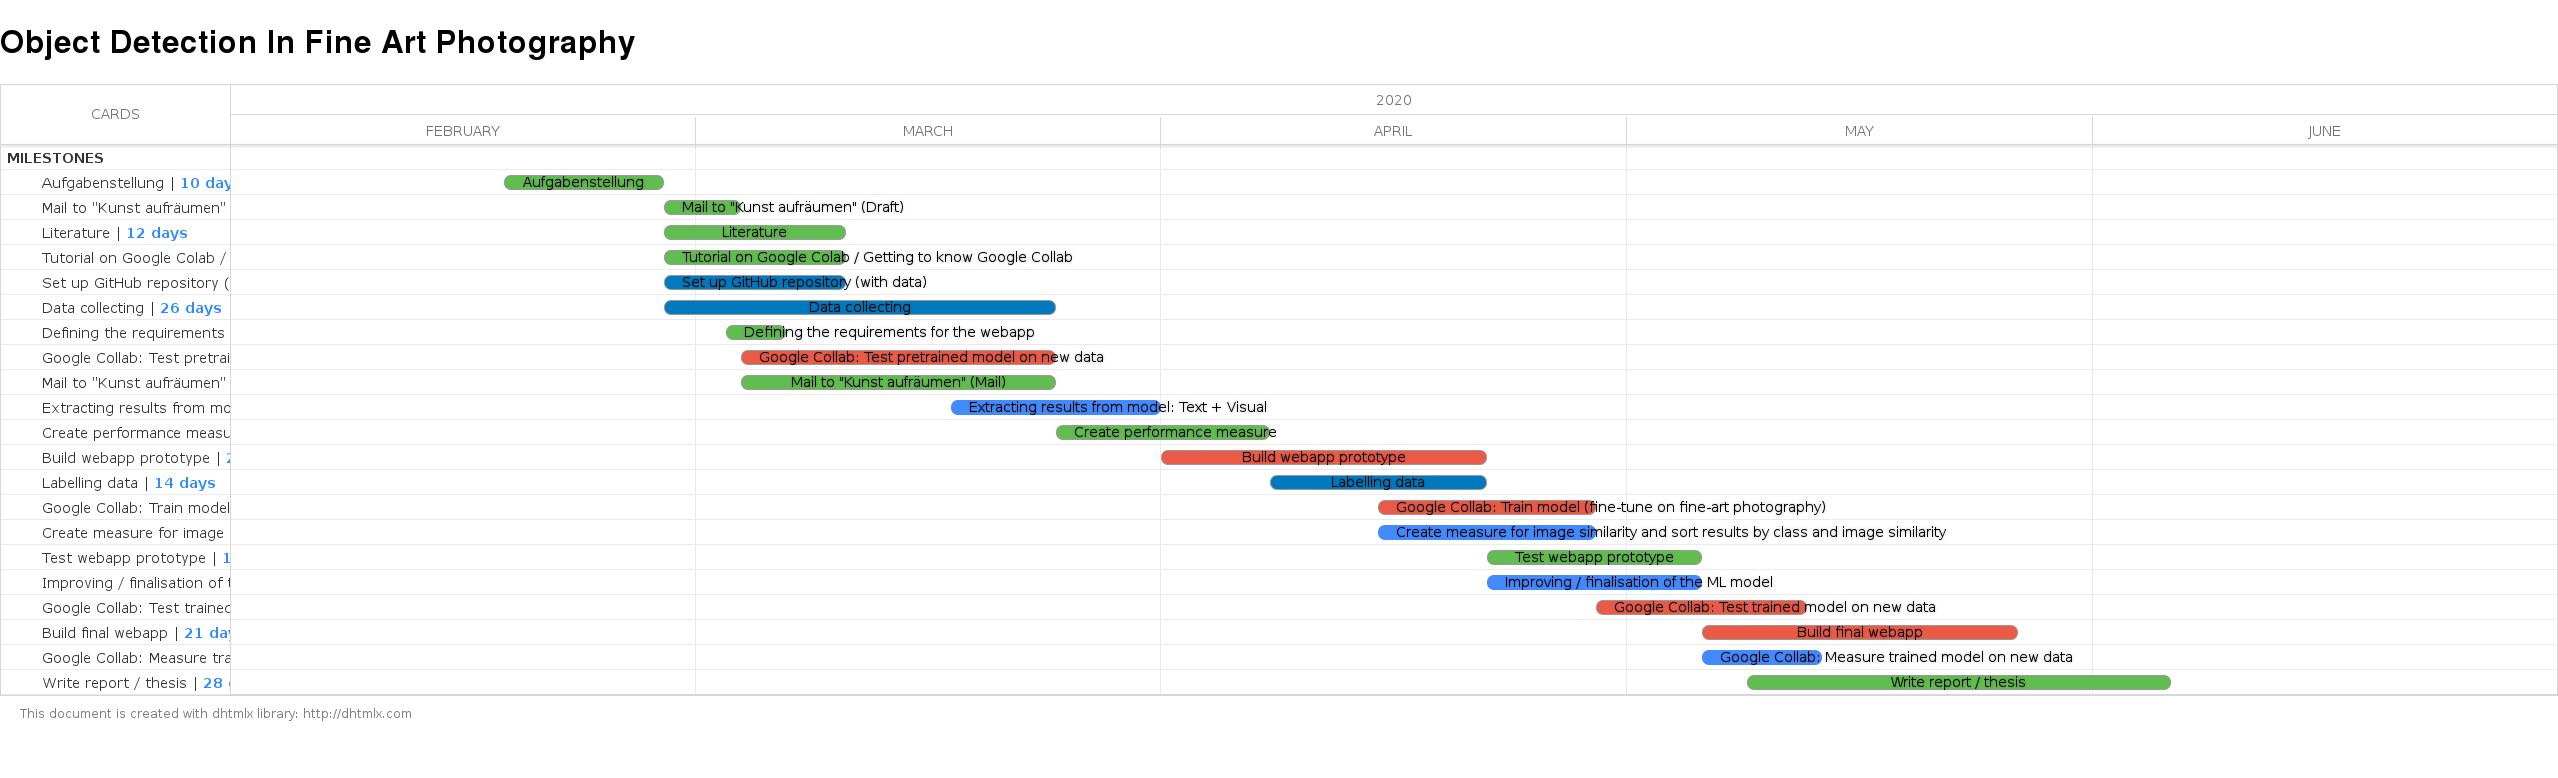
\includegraphics[width=\textwidth]
	{img/project-management-plan.png}}
	\caption{\label{fig:project-management-plan} Timeline view of the project management plan}
\end{figure}

To better structure the project, a number of milestones have been chosen:

\begin{enumerate}
	\item Test pretrained models on Google Colab with new data
	\item Build web application prototype
	\item Finetune model with fine art photography data
	\item Test finetuned model on new data
	\item Finish web application with new model
\end{enumerate}

\section{Codebase}

To develop the project, three different code repositories have been created: A git repository containing different datasets. This repository was used for testing out different models and frameworks when applying inference on the images. When developing the tidied up images, it was used too. It can be reached here: \url{https://gitlab.enterpriselab.ch/iameyer/odifap}.
Another git repository was created to develop the web application. It can be accessed here: \url{https://gitlab.enterpriselab.ch/iameyer/odifap-program}.
The third git repository was created to serve all necessary files for retraining the models. This repository contains a config.py file for every model and a .json file, containing the bounding boxes and masks for retraining.
Large files, like .pth files (checkpoint files, that are generated during training process) were saved to Google drive with the help of a custom Python script.

\section{Testing}

In favour of having more time available for the development cycle and retraining of the model, no testing strategy has been selected.